\chapter{Molecular transport}
\label{ch:transport}

As soon as there are gradients, molecules carry momentum, energy and mass from one place to
another simply by moving randomly. In a flame these fluxes are what bring heat and radicals
\emph{upstream} into the fresh gas and make the flame propagate.

\section{Random walks: where diffusion comes from}

\begin{figure}[H]
\centering
\begin{tikzpicture}
  \draw[thick,fill=gray!5] (0,0) rectangle (8,3);
  \fill[cold!60] (0.3,0.4) circle (2pt);
  \foreach \i in {1,...,70} {\fill[cold!50] ({0.2+3.5*rnd},{0.2+2.6*rnd}) circle (1.3pt);}
  \foreach \i in {1,...,15} {\fill[cold!50] ({3.7+4*rnd},{0.2+2.6*rnd}) circle (1.3pt);}
  \draw[hot,thick,->] (4,1.5) -- (4.5,1.9) -- (4.2,2.4) -- (4.9,2.2) -- (5.3,1.6) -- (4.9,1.1) -- (5.6,0.9);
  \fill[hot] (4,1.5) circle (2pt);
  \node[lbl,hot] at (6.6,0.6) {free path $\ell$};
  \draw[dashed] (4,0) -- (4,3);
  \draw[->,very thick,cold] (3.0,3.4) -- (5.0,3.4) node[midway,above,lbl] {net flux, down the gradient};
  \node[lbl] at (1.8,-0.35) {high concentration};
  \node[lbl] at (6.0,-0.35) {low concentration};
\end{tikzpicture}
\caption{Each molecule moves randomly. More molecules on the left means more random crossings of
the dashed plane from left to right than from right to left. The net flux is down the gradient,
even though no single molecule ``knows'' about it.}
\end{figure}

\begin{derivation}[diffusion coefficient from kinetic theory]
Molecules move at mean speed $\bar c=\sqrt{8k_BT/(\pi m)}$ and travel a \textbf{mean free path}
$\ell=1/(\sqrt2\,n\sigma)$ between collisions ($n$ is number density, $\sigma$ the collision
cross-section). Consider the plane $x=0$ with concentration $C(x)$. Molecules crossing it last
collided about one free path away, so roughly $\tfrac16\bar c\,C(-\ell)$ cross per unit area
left-to-right and $\tfrac16\bar c\,C(+\ell)$ right-to-left (one sixth of directions point along
$+x$). Net flux:
\[
J=\tfrac16\bar c\,[C(-\ell)-C(\ell)]\approx-\tfrac13\bar c\,\ell\,\od{C}{x}
\quad\Longrightarrow\quad D\approx\tfrac13\bar c\,\ell .
\]
Exactly the same argument for momentum and for energy gives the kinematic viscosity
$\nu\approx\tfrac13\bar c\ell$ and the thermal diffusivity $\alpha\approx\tfrac13\bar c\ell$ (up to
factors of order one).
\end{derivation}
\begin{symbols}
$\bar c$ & mean molecular speed $\sqrt{8k_BT/\pi m}$ & \si{\metre\per\second}\\
$m$ & mass of one molecule & \si{\kilo\gram}\\
$\ell$ & mean free path & \si{\metre}\\
$n$ & number density & \si{\per\metre\cubed}\\
$\sigma$ & collision cross-section & \si{\metre\squared}\\
$C(x)$ & concentration of the diffusing species & \si{\kilo\mole\per\metre\cubed}\\
$J$ & net molar flux through the plane & \si{\kilo\mole\per\metre\squared\per\second}\\
$D$, $\nu$, $\alpha$ & mass diffusivity, kinematic viscosity, thermal diffusivity & \si{\metre\squared\per\second}\\
$\mu=\rho\nu$ & dynamic viscosity & \si{\pascal\second}\\
$\lambda=\rho c_p\alpha$ & thermal conductivity & \si{\watt\per\metre\per\kelvin}\\
\end{symbols}

\begin{keypoint}[scalings]
With $\bar c\propto\sqrt{T/m}$ and $\ell\propto1/n\propto T/p$:
\begin{equation}
  D,\ \alpha,\ \nu\;\propto\;\frac{T^{3/2}}{p\,\sqrt m},\qquad
  \mu=\rho\nu\propto\sqrt{T}\ \ (\text{independent of }p),\qquad
  \lambda=\rho c_p\alpha\propto\sqrt{T}.
\end{equation}
Real molecules attract and repel softly (Lennard-Jones potential), which changes the exponents to
roughly $D\propto T^{1.7}/p$ and $\mu,\lambda\propto T^{0.7}$ (\figref{fig:transT}). Three
consequences matter for flames:
\begin{enumerate}
  \item All three diffusivities are of the same order, so $\Pr$ and $\mathrm{Sc}$ are of order one.
  \item Diffusivities scale as $1/p$, so flames get thinner at high pressure.
  \item Light molecules (\ce{H_2}, H) diffuse much faster: $D\propto1/\sqrt m$ (more precisely,
        on the reduced mass of the colliding pair).
\end{enumerate}
\end{keypoint}

\begin{figure}[H]
\centering
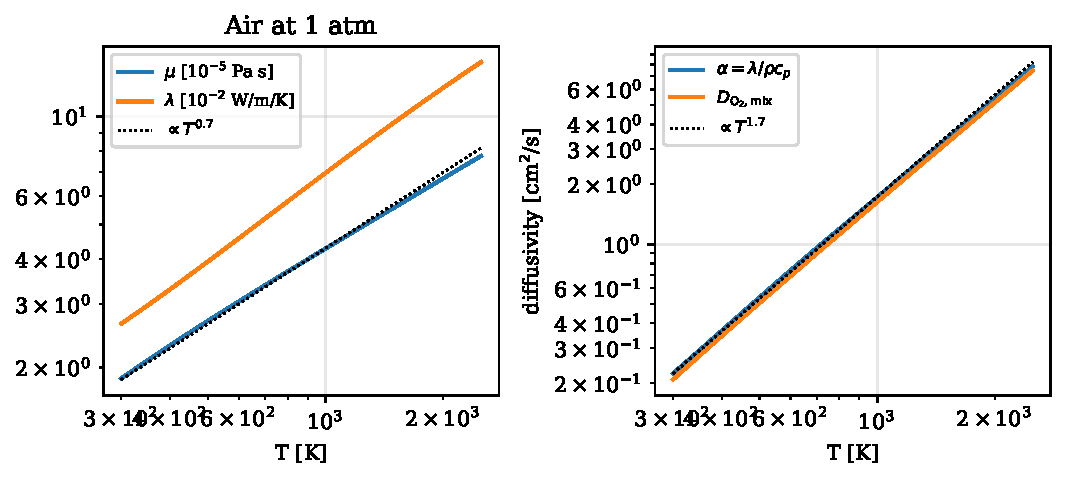
\includegraphics[width=\textwidth]{transport_T}
\caption{Transport properties of air computed by Cantera. Diffusivities grow by a factor of
$\sim20$ between room temperature and flame temperature. This is why the preheat zone of a flame
is much wider on its hot side.}
\label{fig:transT}
\end{figure}

\section{The three flux laws}

\begin{align}
  \text{Newton (momentum):}\quad &\tau_{ij}=\mu\Big(\pd{u_i}{x_j}+\pd{u_j}{x_i}\Big)-\tfrac23\mu\,\delta_{ij}\,\divg\vu,\\
  \text{Fourier (heat):}\quad &\vq=-\lambda\nabla T+\sum_kh_k\vj_k\quad(+\text{Dufour, negligible}),\\
  \text{Fick (species):}\quad &\vj_k=\rho Y_k\vV_k\approx-\rho D_{k}\nabla Y_k .
  \label{eq:fick}
\end{align}

\begin{symbols}
$\tau_{ij}$ & viscous stress component & \si{\pascal}\\
$\mu$ & dynamic viscosity & \si{\pascal\second}\\
$u_i$, $x_i$ & velocity component, coordinate & \si{\metre\per\second}, \si{\metre}\\
$\delta_{ij}$ & Kronecker delta (1 if $i=j$, else 0) & \nodim\\
$\vq$ & heat flux & \si{\watt\per\metre\squared}\\
$\lambda$ & thermal conductivity & \si{\watt\per\metre\per\kelvin}\\
$h_k$ & specific enthalpy of $k$ & \si{\joule\per\kilo\gram}\\
$\vj_k$, $\vV_k$ & diffusive mass flux, diffusion velocity of $k$ & \si{\kilo\gram\per\metre\squared\per\second}, \si{\metre\per\second}\\
$D_k$ & diffusivity of $k$ & \si{\metre\squared\per\second}\\
\end{symbols}
$\vV_k$ is the \textbf{diffusion velocity} of species $k$ relative to the mass-averaged velocity
$\vu$, and $\vj_k$ the diffusive mass flux. The $\sum h_k\vj_k$ term in $\vq$ is
enthalpy carried by species diffusing: a hot H atom diffusing upstream brings its enthalpy along.

\begin{derivation}[the mass-conservation constraint]
$\vu$ is defined as the mass-averaged velocity, $\rho\vu=\sum_k\rho Y_k\vu_k$. Hence the diffusive fluxes
must add up to zero:
\begin{equation}
  \sum_k\vj_k=\sum_k\rho Y_k\vV_k=0 .
\end{equation}
Fick's law with arbitrary $D_k$ violates this. Practical codes, including Cantera, add a
\textbf{correction velocity} $\vV_c=-\sum_kY_k\vV_k^{\rm Fick}$ to every species so that the sum
is zero.
\end{derivation}
\begin{symbols}
$\vu$ & mass-averaged velocity & \si{\metre\per\second}\\
$\vu_k$ & velocity of species $k$ & \si{\metre\per\second}\\
$\vV_k=\vu_k-\vu$ & diffusion velocity of $k$ & \si{\metre\per\second}\\
$\vV_c$ & correction velocity added to every species & \si{\metre\per\second}\\
$\vj_k=\rho Y_k\vV_k$ & diffusive mass flux of $k$ & \si{\kilo\gram\per\metre\squared\per\second}\\
\end{symbols}

\section{Mixture-averaged and multicomponent diffusion}

Kinetic theory gives binary coefficients $\mathcal D_{jk}$ for each pair of species. In a
mixture, species $k$ collides with everything. Two models:
\begin{itemize}
  \item \textbf{Mixture-averaged} (Cantera \code{"mixture-averaged"}, the default): $k$ diffuses into
        an effective ``rest of the mixture'' with
        \begin{equation}
          D_{km}=\frac{1-Y_k}{\sum_{j\ne k}X_j/\mathcal D_{jk}},\qquad
          \vj_k=-\rho\frac{W_k}{W}D_{km}\nabla X_k+\rho Y_k\vV_c .
        \end{equation}

\begin{symbols}
$D_{km}$ & mixture-averaged diffusivity of $k$ & \si{\metre\squared\per\second}\\
$\mathcal D_{jk}$ & binary diffusivity of the pair $j$--$k$ & \si{\metre\squared\per\second}\\
$X_j$, $Y_k$ & mole, mass fractions & \nodim\\
$W_k$, $W$ & molar mass of $k$, of the mixture & \si{\kilo\gram\per\kilo\mole}\\
$\vV_c$ & correction velocity & \si{\metre\per\second}\\
\end{symbols}
        Cheap and accurate to a few percent for most flames.
  \item \textbf{Multicomponent} (\code{"multicomponent"}): solves the full Stefan--Maxwell relations
        $\nabla X_k=\sum_j\frac{X_kX_j}{\mathcal D_{kj}}(\vV_j-\vV_k)+\dots$, plus
        \textbf{thermal diffusion} (Soret effect: light species are pushed towards hot regions).
        More expensive. It matters for \ce{H_2} and H, especially in lean \ce{H_2} flames.
\end{itemize}
\begin{lstlisting}
flame.transport_model = "mixture-averaged"     # default
flame.transport_model = "multicomponent"; flame.soret_enabled = True
flame.transport_model = "unity-Lewis-number"   # D_k = alpha for every k
\end{lstlisting}

\paragraph{Mixture viscosity and conductivity} come from species values with mixing rules
(Wilke's formula for $\mu$, an average of arithmetic and harmonic means for $\lambda$). Cantera does
this for you from the Lennard-Jones parameters stored for each species in the YAML file.

\section{Dimensionless numbers}

Making the governing equations dimensionless with a length $L$, velocity $U$ and the property
values produces ratios that say which process dominates:
\begin{table}[H]
\centering
\begin{tabular}{llll}
\toprule
number & definition & compares & typical (flame) \\
\midrule
Reynolds & $\mathrm{Re}=UL/\nu$ & inertia / viscous diffusion & laminar: $<\!\sim\!10^3$ \\
Prandtl & $\Pr=\nu/\alpha$ & momentum / heat diffusion & $\approx0.7$ \\
Schmidt & $\mathrm{Sc}_k=\nu/D_k$ & momentum / mass diffusion & 0.2 (\ce{H_2}) -- 1.5 \\
\textbf{Lewis} & $\mathrm{Le}_k=\alpha/D_k$ & \textbf{heat / mass diffusion} & 0.3 (\ce{H_2}) -- 2 \\
\bottomrule
\end{tabular}
\end{table}

\begin{figure}[H]
\centering
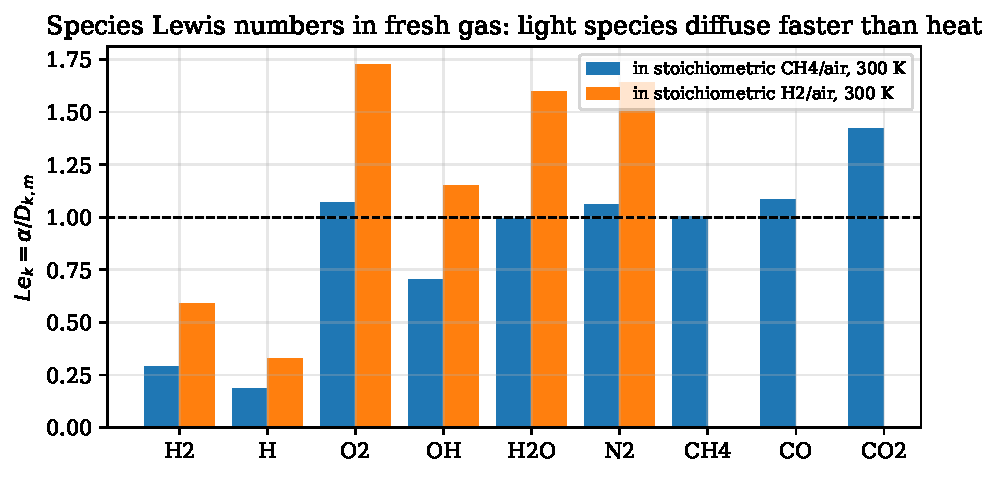
\includegraphics[width=0.9\textwidth]{lewis}
\caption{Lewis numbers in fresh stoichiometric gas. \ce{H_2} and especially H diffuse much faster
than heat ($\mathrm{Le}<1$). \ce{CH_4}, \ce{O_2} and \ce{N_2} are close to 1.}
\label{fig:lewis}
\end{figure}

\begin{figure}[H]
\centering
\begin{tikzpicture}
  \begin{scope}
    \shade[inner color=hot!60,outer color=white] (0,0) circle (1.2);
    \shade[inner color=cold!60,outer color=white,opacity=0.6] (0,0) circle (1.2);
    \fill (0,0) circle (1.5pt);
    \node[lbl,align=center] at (0,-1.7) {$\mathrm{Le}=1$:\\heat and fuel spread together};
  \end{scope}
  \begin{scope}[xshift=5cm]
    \shade[inner color=cold!60,outer color=white,opacity=0.8] (0,0) circle (1.6);
    \shade[inner color=hot!70,outer color=white,opacity=0.8] (0,0) circle (0.8);
    \fill (0,0) circle (1.5pt);
    \node[lbl,align=center] at (0,-1.9) {$\mathrm{Le}<1$ (\ce{H_2}):\\fuel spreads faster than heat};
  \end{scope}
  \node[lbl,hot] at (7.4,0.6) {heat};
  \node[lbl,cold] at (7.4,-0.2) {fuel};
\end{tikzpicture}
\caption{Lewis number as a race between heat and species. With $\mathrm{Le}<1$ a reacting region
draws in fuel faster than it loses heat, so it becomes richer and hotter locally. This is
\textbf{preferential diffusion}.}
\label{fig:lerace}
\end{figure}

\section{The unity-Lewis-number simplification}
\label{sec:unityLe}

\begin{derivation}[enthalpy becomes a conserved scalar when all $\mathrm{Le}_k=1$]
Take the heat flux with Fick's law, $\vq=-\lambda\nabla T-\sum_kh_k\rho D_k\nabla Y_k$. Since
$h=\sum_kY_kh_k(T)$,
\[
\nabla h=c_p\nabla T+\sum_kh_k\nabla Y_k
\quad\Longrightarrow\quad
\lambda\nabla T=\frac{\lambda}{c_p}\nabla h-\frac{\lambda}{c_p}\sum_kh_k\nabla Y_k .
\]
Substituting,
\begin{equation}
  \vq=-\rho\alpha\nabla h+\sum_kh_k\,\rho\,(\alpha-D_k)\nabla Y_k .
\end{equation}
If $D_k=\alpha$ for every species ($\mathrm{Le}_k=1$), the sum vanishes and $\vq=-\rho\alpha\nabla
h$. The enthalpy equation of \chapref{ch:governing} (low Mach number, no radiation) becomes
\[
\rho\Dt{h}=\divg(\rho\alpha\nabla h),
\]
which has no source term: $h$ is transported like a passive dye. By the same argument, every
\emph{elemental} mass fraction (and therefore the mixture fraction, \chapref{ch:nonpremixed}) is
conserved, because chemistry rearranges atoms but never creates them.
\end{derivation}
\begin{symbols}
$\vq$ & heat flux & \si{\watt\per\metre\squared}\\
$\lambda$ & thermal conductivity & \si{\watt\per\metre\per\kelvin}\\
$h$, $h_k$ & specific enthalpy of mixture, of species $k$ & \si{\joule\per\kilo\gram}\\
$c_p$ & specific heat capacity & \si{\joule\per\kilo\gram\per\kelvin}\\
$\alpha=\lambda/\rho c_p$ & thermal diffusivity & \si{\metre\squared\per\second}\\
$D_k$ & diffusivity of species $k$ & \si{\metre\squared\per\second}\\
$\mathrm{Le}_k=\alpha/D_k$ & Lewis number of species $k$ & \nodim\\
$\nabla T$, $\nabla Y_k$ & temperature and mass-fraction gradients & \si{\kelvin\per\metre}, \si{\per\metre}\\
\end{symbols}

\begin{keypoint}
With unity Lewis numbers, enthalpy and element mass fractions are linear functions of the mixture
fraction in a two-stream problem. That makes the equilibrium temperature $T_{\rm eq}(Z)$
meaningful (Part~2) and keeps the mixture fraction constant through a premixed flame (Part~3).
With real (mixture-averaged) transport and $\mathrm{Le}_{\ce{H_2}}\approx0.3$, both statements break.
The size of the breakage is exactly what Part~3, Task~3 asks you to measure.
\end{keypoint}

\begin{selfcheck}
\begin{enumerate}
  \item Doubling the pressure: what happens to $D$, $\mu$ and to a flame's thickness?
  \item Why is $\mathrm{Le}_{\rm H}$ even smaller than $\mathrm{Le}_{\ce{H_2}}$?
  \item Under $\mathrm{Le}=1$, can the local enthalpy inside a flame differ from the fresh-gas
        enthalpy? And under mixture-averaged transport?
\end{enumerate}
\end{selfcheck}
